\documentclass[12pt, preprint]{aastex}
\usepackage{bm}
\usepackage{amsmath}


\newcommand{\setof}[1]{\left\{{#1}\right\}}
\newcommand{\given}{\,|\,}
\newcommand{\dd}{\mathrm{d}}
\newcommand{\catalog}{\bm{Q}}
\newcommand{\pars}{\bm{\theta}}
\newcommand{\amin}{\ifmmode {^{\prime}\ }\else$^{\prime}$\fi}
\newcommand{\asec}{\ifmmode {^{\prime\prime}}\else$^{\prime\prime}$\fi}
\newcommand{\bs}[1]{\boldsymbol{#1}}

\newcommand{\Msun}{\ifmmode {M_{\odot}}\else${M_{\odot}}$\fi}
\newcommand{\Porb}{\ifmmode {P_{\rm orb}}\else${P_{\rm orb}}$\fi}

\begin{document}

\title{An alternative to binary population synthesis: \\ Correlating X-ray populations with star forming regions}
%\title{Modeling the X-Ray Populations of the LMC}
\author{some combination of JJA, AZ, TF, and others}
\date{NOT READY}

\begin{abstract}
Population models typically require a large number of simulation realizations, a computationally expensive endeavor, to generate statistically robust results. Employing Monte Carlo importance sampling, population synthesis offers a substantial improvement over brute force grid-based studies. However for certain problems, particularly those with a large dimensionality, even population synthesis is limited by computational expense. We describe a novel approach which uses a Markov Chain Monte Carlo technique instead of population synthesis to model individual elements in a population. Our technique is derived for stellar binaries, but can, in principle, be applied to any population. We test our method on a 10-dimensional model for the population of high mass X-ray binaries in the LMC, and successfully recover input parameters for two synthetic binaries. We apply our model to one particular system. Finally, we discuss future directions for this method. In the era of gravitational wave astronomy, efficient methods are needed to derive evolutionary histories for individual binary systems.
\end{abstract}





\section{Introduction}


The space-based X-ray observatory {\it Chandra} has revolutionized our understanding of X-ray luminous objects. Its unprecedented angular precision and collecting area allows it to identify dozens of resolved sources in nearby galaxies (references). Studies of individual objects have yielded a deeper insight into the physical processes forming the bulk of individually identified sources, low and high mass X-ray binaries, as well as a rare, but important subset, the ultra-luminous X-ray sources (references). High mass X-ray binaries (HMXB), in particular, are formed from the accretion of an early-type star onto either a neutron star or black hole (van den Heuvel?). Their relatively short lifetimes require that these systems cannot travel far away from their birth site, and indeed observations show that many of luminous X-ray sources are near star forming regions \citep{zezas02, kaaret04}. 

The nearby Small and Large Magellanic Clouds have the best studied extragalactic X-ray populations. Long term X-ray campaigns with {\it Chandra} have identified every X-ray emitting object with $L_x < 10^{32}$ erg s$^{-1}$ in the SMC, and ongoing observations of the somewhat larger LMC are approaching this degree of sensitivity (Zezas, Laycock et al.). At the same time, infrared, optical, and ultraviolet imaging with {\it HST} provide detailed spatially resolved star formation histories of the SMC and LMC with angular resolutions as small as 12\amin\ by 12\amin\ regions (Harris \& Zaritsky). These star formation histories are precise, particularly so over the past 10$^8$ yr when HMXBs were formed.


So far, models comparing regions of past star formation and the observed population of HMXBs have focused on the distance a population of HMXBs are expected to travel as a function of time \citep{sepinsky05} and how the distance can affect binary characteristics such as orbital period and X-ray luminosity \citep{zuo10, zuo15}. These models all employ population synthesis techniques.


Population studies typically seek to compare the likelihood of individual models to fit some set of astrophysical objects. Previous analysis of binary star populations have primarily relied on population synthesis, in which one randomly generates, according to some predetermined initial distribution of parameters, a large number of stellar binaries. By including our best understanding of binary evolution, this population is then evolved until its present state, when one then takes a ``snapshot'' of the binaries to determine the resulting population at a given time. %Finally, to compare to an observational sample, any observational biases must be included in the model. 


Discussion of StarTrack, Biceps, SeBa, BSE, others. Include general method and results. Reference comparison paper?


Yet, population synthesis is not the only method to populations of stars, and for rare or short-lived evolutionary states, it is exceedingly poor; significant computational time is spent on regions of parameter space of no interest to the observed systems. For HMXBs, specifically, mass transfer and supernova kicks may merge or disrupt the majority of systems. Therefore, in many binary population synthesis studies, $10^6-10^7$ binaries are required to make statistically robust comparisons with observed populations. An alternative is wanting.


Bhadkamkar \& Ghosh (2012) presented an alternative to population synthesis for HMXBs in which they analytically transformed the initial binary conditions 


 Instead of treating the kick velocity as a three-dimensional distribution, they applied the maximum likelihood value to a binary, reducing the marginalization in Equation \ref{eq:bayes} to a three-dimensional integral (the two initial masses and binary separation). Using Jacobian transformations, these authors analytically represented the current state of HMXBs as transformations of the initial conditions of a binary; they could determine exactly which initial conditions produced HMXBs with specific $L_x$. Subsequent integration over the remaining two parameters provided an X-ray luminosity function. However, this method was wanting in two separate aspects. First, their treatment of the SN kick velocity is an approximation, since they do not apply a distribution of kick velocities. Second, their analysis did not include the evolution over time. 






%at to characterize the population of HMXBs at a given time. By comparing the observed population of HMXBs in the SMC to the simulation ``snapshot'' after 60 Myr (the most recent ''starburst'' in the SMC), one can estimate the accuracy of our understanding of binary evolution. In essence population synthesis is a Monte Carlo numerical solution to the integral for the observed HMXBs:

In this work, we model the formation of HMXBs in a novel way using a Markov Chain Monte Carlo technique which naturally focuses computational power is on the region of parameter space relevant of interest. This method is versatile and substantially more efficient than comparable population synthesis methods, however care must be taken to properly normalize this prior distributions. 



In Section 2 we describe our method and show that it is mathematically equivalent to standard population synthesis. In Section 3 we discuss our implementation of single star and binary evolution and how we calculate the priors based on star formation history. We apply our method to two synthetic test HMXB as well as the pulsar binary J0045-7319 in Section 4. Finally, we provide some conclusions and future applications of this method in Section 5.







\begin{comment}

We augment the problem to nine dimensions, adding the position and birth time as components of $\vec{x}_i$. Because of both its well characterized HMXB population and its precise star formation history, the LMC is an excellent testbed for this method. We apply our 9-parameter model to each HMXBs in the sample. Our results provide important constraints on both the binaries forming of each of these systems and the HMXB population of the LMC as a whole.

%NGC 55 is a relatively transparent, edge-on, nearby galaxy. Using the {\it Hubble Space Telescope}, and other optical telescopes, we have been able to identify a near-complete sample of star forming regions. For each region, multi-band photometry provides an estimate of the star formation history. 


%simulate the expected number, position, and characteristics of the X-ray binary population, given our sample of star forming regions, as well as the star formation history of the overall galaxy. We then apply a Bayesian method to generate a likelihood function comparing the resulting distribution with the observed X-ray sample.


\end{comment}



\section{Statistical Method}

We first describe the mathematical foundation behind using MCMC for population synthesis studies. Population studies typically seek to compare the likelihood of individual models to fit some set of astrophysical objects. We are interested in calculating the probability of the data given some model, $P(D \given M)$. If we want to compare an observed population to different models, we may be interested in determining the inverse quantity, $P(M \given D)$. These two quantities can be linked using Bayes' formula:
\begin{equation}
P(M \given D) = \frac{P(D \given M) P(M)}{P(D)}, \label{eq:bayes}
\end{equation}
where $P(M)$ is the prior probability on the model, $P(D)$ is the so-called evidence, and $P(D \given M)$ is the likelihood of the data given the model. 
%Two likelihood of two separate models can be then be compared straightforwardly:
%\begin{equation}
%\frac{P(M_1 \given D)}{P(M_2 \given D)} = \frac{P(D \given M_1)}{P(D \given M_2)} \frac{P(M_1)}{P(M_2)}.
%\end{equation}

For most problems, we cannot calculate $P(D \given M)$ directly, but must instead marginalize over a set of parameters ($\vec{x}$) with known distributions. Here, we will marginalize over two sets of parameters, $\vec{x}_i$ and $\vec{x}_f$, representing the initial and final states of the binary, respectively:
\begin{equation}
P(D \given M) = \int \dd \vec{x}_i\ \dd \vec{x}_f\ P(D \given \vec{x}_f, M)\ P(\vec{x}_f \given \vec{x}_i, M)\ P(\vec{x}_i \given M). \label{eq:bayes_marginalize}
\end{equation}
For stellar binaries $P(\vec{x}_i \given M)$ represents the initial binary distributions, and $P(\vec{x}_f \given \vec{x}_i, M)$ is calculated from the binary evolution routines that evolve a binary from an initial state to its state today, and $P(D \given \vec{x}_f, M)$ accounts for the observations of the system, including uncertainties and biases.

To calculate this multidimensional integral, binary population synthesis uses importance sampling:
\begin{equation}
\int \dd \vec{x}_i\ \dd \vec{x}_f\ P(D \given \vec{x}_f, M)\ P(\vec{x}_f \given \vec{x}_i, M)\ P(\vec{x}_i \given M) \approx \frac{V}{N} \sum_{j \in N} P(D \given \vec{x}_f, M)\ P(\vec{x}_f \given \vec{x}_{i,j}, M), \label{eq:pop_synth}
\end{equation}
where $\vec{x}_{i,j}$ are drawn from their probability distributions:
\begin{equation}
\vec{x}_{i,j} \sim P(\vec{x}_i \given M).
\end{equation}
%For an infinite number of random draws, the approximation in Equation \ref{eq:pop_synth} becomes an equality. 
For binary populations involving neutron stars (NS) and black holes (BH), population synthesis may be an inefficient tool; common envelope evolution and supernova kicks may merge or disrupt the majority of systems before they evolve into objects of interest (mathematically, $P(\vec{x}_f \given \vec{x}_{i,j}, M) = 0$ for many or even most of the randomly drawn $\vec{x}_i$). In many binary population synthesis studies, $10^6-10^7$ binaries are required to make statistically robust comparisons with observed populations.

Here, we demonstrate an alternative method, in which the integral in which random $D_j$ are directly drawn based on the entire quantity in the integrand in Equation \ref{eq:bayes_marginalize}:
\begin{equation}
\vec{D}_j \sim P(D \given \vec{x}_f, M)\ P(\vec{x}_f \given \vec{x}_i, M)\ P(\vec{x}_i \given M). 
\end{equation}
Equation \ref{eq:bayes_marginalize} is then calculated using a Markov Chain Monte Carlo technique:
\begin{equation}
P(D \given \vec{x}_f, M)\ P(\vec{x}_f \given \vec{x}_i, M)\ P(\vec{x}_i \given M) \approx \frac{V}{N} \sum_{j \in N} P(D_j). \label{eq:MCMC}
\end{equation}

In this method, every component of $\vec{x}_i$ is a model parameter. $P(\vec{x}_i \given M)$ is the prior probability on $\vec{x}$ and $P(D \given \vec{x}_f, M)\ P(\vec{x}_f \given \vec{x}_i, M)$ is the likelihood function. We cannot directly generate a large sample of $D_j$. Instead, MCMC provides an algorithm that probes the $\vec{x}_i$ parameter space incrementally to create a sample. For binary evolution, in which $P(D \given \vec{x}, M)$ has substantial structure, this form can be substantially more efficient, since substantially less computational time is spent evolving systems outside the parameter space region of interest. The cost of this method is additional overhead in the process, since the likelihood must be calculated at every step, for every $\vec{x}_i$, before the next $\vec{x}_i$ can be chosen.






\begin{comment}
Mathematically, population synthesis seeks to Monte Carlo-generate observations ($obs$) by drawing from $P(obs)$. Since we cannot know $P(obs)$ a priori, we instead calculate it by marginalizing over initial binary distributions ($\vec{x}$):
\begin{equation}
P(obs) = \int \dd \vec{x}\ P(obs \given \vec{x})\ P(\vec{x} ). \label{eq:bayes}
\end{equation}
$P(obs \given \vec{x}_i)$ contains the evolution of the binary and any observational biases that may exist. Since the integration in Equation \ref{eq:bayes} may be over a large dimensional space, standard numerical techniques cannot be efficiently applied, and population synthesis provides a straightforward solution to the problem. By drawing randomly from these initial distributions, traditional population synthesis makes the approximation:
\begin{equation}
P(obs) \approx \frac{V}{N} \sum_{i \in N} P(obs \given \vec{x}_i), \label{eq:pop_synth}
\end{equation}
where random $\vec{x}_i$ are drawn from $P(\vec{x})$. 
\end{comment}



\subsection{High Mass X-ray Binaries - Population}

Our goal is to identify quantitatively how a population of HMXBs formed. We begin with Bayes' Rule:
\begin{equation}
P( \vec{x}_i \given D, M ) = \frac{P( D \given M, \vec{x}_i ) P(\vec{x}_i \given M)}{P(D \given M)},
\end{equation}
where $\vec{x}_i$ are the binary parameters described above, $M$ is the binary evolution model and $D$ contains the observed data. To simulate an HMXB population, $D$ may be an X-ray bright object, quantified as an accreting binary with an $L_x$ above some observationally-motivated threshold. To first order HMXBs can be determined uniquely by its initial masses, $M_{1,i}$ and $M_{2,i}$, its initial binary separation, $a_i$, and eccentricity $e_i$, and the kick velocity it received after the primary collapsed to form a NS or BH, $\vec{v}_k$. For the problem at hand, we also include the binary's birth position, $\alpha_i$ and $\delta_i$, and its birth time, $t_i$:
\begin{equation}
\vec{x}_i \in ( M_{1,i}, M_{2,i}, a_i, e_i, \vec{v}_k, \alpha_i, \delta_i, t_i ). \label{eq:x_i}
\end{equation}

In this case, calculating the integrand in Equation \ref{eq:bayes_marginalize} is straightforward; $P(obs \given \vec{x}_i)$ are the priors which we discuss in Section \ref{sec:priors} and $P(obs \given \vec{x})$ ensures that only HMXBs are selected (unity for accreting binaries, and zero for non-accreting binaries).



\subsection{High Mass X-ray Binaries - Individual Systems}

In our model we simulate individual HMXBs using the same model parameters as we use for a population, so $\vec{x}_i$ is determined by Equation \ref{eq:x_i}. However, HMXBs in the SMC and LMC may have well measured $P'_{\rm orb}$, $e'$, and $M'_2$ determined from identifying the observational counterpart to the X-ray source. Each of these measured quantities has some uncertainty associated with it. Furthermore, individual HMXBs have a specific location that we are trying to associate with nearby star forming regions. Therefore, the likelihood function in Equation \ref{eq:bayes_marginalize} is somewhat more complicated. We start by defining $D$ as:
\begin{equation}
D \in (\alpha, \delta, P'_{\rm orb}, e', M'_2). \label{eq:D}
\end{equation}
We use primed quantities to denote observed values that are, in general, different from the true, physical values $P'_{\rm orb}$, $e'$, and $M'_2$. We ignore uncertainties on the position.


To generate our likelihood function, we now marginalize over four parameters, the true orbital parameters, $P_{\rm orb}$ and $e$, the true (current) companion mass $M_2$, and the systemic velocity ($v_{\rm sys}$):
\begin{equation}
P(D \given \vec{x}_i, M) =  \int \dd P_{\rm orb}\ \dd e\ \dd M_2\ \dd v_{\rm sys}\ P( P_{\rm orb}, e, M_2, v_{\rm sys}, D \given \vec{x}_i, M).
\end{equation}
Based on independence, we express this integral into separate, tractable parts:
\begin{eqnarray}
P(D \given M, \vec{x}_i) &=&  \int \dd P_{\rm orb}\ \dd e\ \dd M_2\ \dd v_{\rm sys}\ P(P'_{\rm orb} \given P_{\rm orb}) \nonumber \\
	& & \qquad \times P(e' \given e)\ P(M'_2 \given M_2) \nonumber \\
	& & \qquad \times P(\alpha, \delta \given \alpha_i, \delta_i, t_i, M_{1,i}, v_{\rm sys}) \nonumber \\
	& & \qquad \times P(P_{\rm orb}, e, M_2, v_{\rm sys} \given M_{1,i}, M_{2,i}, a_i, e_i, \vec{v}_k, t_i). \label{eq:marginalized}
\end{eqnarray}
The two terms in the integrand, $P(P'_{\rm orb} \given P_{\rm orb})$ and $P(e' \given e)$, include the observational uncertainties on the binary's orbit. We model these with Gaussian uncertainties, but in principle, can account for any observationally-derived distribution. Similarly, $P(M'_2 \given M_2)$ accounts for the observational uncertainty on $M_2$. This term again can be approximated as a Gaussian distribution, but a more careful determination will include a comparison between the observed magnitudes in various filters and stellar models on a color-magnitude diagram. 

The fourth term in the integrand accounts for the fact that the system's birth place may, in general, be different from its observed position since the center of mass of a system received a kick during the primary's core collapse. We explicitly include dependencies on $v_{\rm sys}$, $t_i$, and $M_{1,i}$ since the distance travelled depends on both the system's velocity and time since the primary's supernova. We derive this term in Section \ref{sec:ra_dec} below. 

The last term of the integrand, which we discuss in Section \ref{sec:binary_evolve}, includes the binary evolution from its {\it ab initio} state to the $P_{\rm orb}$, $e$, $M_2$, and $v_{\rm sys}$ of the system today. In section \ref{sec:priors} we derive the prior distributions for each of our ten model parameters.



\subsubsection{Position Probability: $P( \alpha, \delta \given \alpha_i, \delta_i, t_i, M_{1,i}, v_{\rm sys} )$} \label{sec:ra_dec}

The first term provides the probability that, given a system's birth time, position, systemic velocity, and initial primary mass, the system would be observed at its current position. Since HMXBs are generally short lived, this probability is non-zero for only a small region around any given HMXB's observed position. To solve the positional component of Equation \ref{eq:marginalized}, we first marginalize over $\omega$ the angle between the line of sight vector to the birth location and the systemic velocity vector:
\begin{equation}
P(\alpha, \delta \given \alpha_i, \delta_i, t_i, M_{1,i}, v_{\rm sys} ) = \int \dd \omega\ P(\alpha, \delta, \omega \given \alpha_i, \delta_i, t_i, M_{1,i}, v_{\rm sys} ). \label{eq:P_pos_1}
\end{equation}

\begin{figure}[h!]
\begin{center}
\includegraphics[width=0.95\columnwidth]{../figures/position_projected.pdf}
\caption{Our representation of the current position $(\alpha, \delta)$ in relation to its birth position $(\alpha_i, \delta_i)$. The distance the system traveled is $d$, which has a projected separation $s$. We express this transportation as a function of $\theta_{\rm proj}$ and position angle, $\phi$. Note, for typical systems $d << D_{\rm LMC}$.}
\label{fig:position_projection}
\end{center}
\end{figure}


We next perform a coordinate transform from the absolute positional coordinates $\alpha$ and $\delta$ to the angular separation, $\theta_{\rm proj}$, and the position angle, $\phi$, measured from the system's birth location. The determinant of the Jacobian matrix for this transformation is:
\begin{equation}
J_{\rm coor} = \left| \frac{\dd \alpha}{\dd \theta_{\rm proj}} \frac{\dd \delta}{\dd \phi} - \frac{\dd \alpha}{\dd \phi} \frac{\dd \delta}{\dd \theta_{\rm proj}} \right|.
\end{equation}
Equation \ref{eq:P_pos_1} now becomes:
\begin{eqnarray}
P(\alpha, \delta \given \alpha_i, \delta_i, t_i, M_{1,i}, v_{\rm sys} ) &=& \int \dd \omega\ P(\theta_{\rm proj}, \phi, \omega \given t_i, M_{1,i}, v_{\rm sys} ) J_{\rm coor}. \nonumber \\
&=& \int \dd \omega\ P(\theta_{\rm proj} \given \omega,  t_i, M_{1,i}, v_{\rm sys} )\ P(\phi)\ P(\omega)\ J_{\rm coor}, \label{eq:P_pos_2}
\end{eqnarray}
where we have separated terms based on independence; $\omega$ is a randomly chosen polar angle and $\phi$ is a randomly chosen azimuthal angle with normalized probabilities, respectively: 
\begin{eqnarray}
P(\omega) &=& \frac{\sin \omega} {2}, \in [0,\pi] \\
P(\phi) &=& \frac{1}{2 \pi}, \in [0, 2\pi].
\end{eqnarray}


The physical distance an HMXB travels is the product of $v_{\rm sys}$ and the time since the primary's core collapse:
\begin{equation}
d = v_{\rm sys} \left[t_i - t(M_{1,i}) \right],
\end{equation}
where $t(M_{1,i})$ is the lifetime of a star with a mass of $M_{1,i}$. We can only observe the projection of $d$ onto the sky, $s = d \sin \omega$. $s$ is approximated as the product of the distance to the LMC, $D_{\rm LMC}$ and $\theta_{\rm proj}$, which allows us to express $\theta_{\rm proj}$ in terms of model parameters:
\begin{equation}
\theta_{\rm proj} = \frac{v_{\rm sys} \left[ t_i - t(M_{1,i}) \right] \sin \omega}{D_{\rm LMC}}. \label{eq:theta_proj}
\end{equation}
The third term in the integrand in Equation \ref{eq:P_pos_2} is a delta function:
\begin{equation}
P(\theta_{\rm proj} \given \omega, t_i, M_{1,i}, v_{\rm sys}) = \delta \left[G(\omega)\right], \label{eq:P_theta_proj}
\end{equation}
where:
\begin{equation}
G(\omega) = \theta_{\rm proj} - \frac{v_{\rm sys} \left[t_i - t(M_{1,i}) \right] \sin \omega}{D_{\rm LMC}}.\end{equation}


With the delta function from Equation \ref{eq:P_theta_proj}, the integral in Equation \ref{eq:P_pos_2} can be reduced:
\begin{equation}
\int \dd \omega\ P(\phi) P(\omega) \delta \left[ G(\omega) \right]  J_{\rm coor}\  =\ \sum_i\ \frac{P(\omega_i^{\star}) P(\phi)  J_{\rm coor}}{ \left| \frac{ \dd G (\omega) }{\dd \omega} \right|_{\omega_i^*}},
\end{equation}
where $G(\omega)$ is the function inside the delta function in Equation \ref{eq:P_theta_proj} and the sum is over $\omega_i^*$, the $i$ roots of $G(\omega)$. There are two roots corresponding to whether the object is in front of or behind its birth location. This integral can now be evaluated analytically:
\begin{equation}
P(\alpha, \delta \given \alpha_i, \delta_i, t_i, M_{1,i}, v_{\rm sys} ) =
\begin{cases} 
      0, & \theta_{\rm proj} \geq \theta_C\\
     \frac{\tan \omega^*}{2 \pi \theta_C}  J_{\rm coor}, & \theta_{\rm proj} < \theta_C 
   \end{cases}
\end{equation}
where:
\begin{equation}
\omega^{\star} = \sin^{-1} \left[ \frac{\theta_{\rm proj}}{\theta_C} \right].
\end{equation}
and
\begin{equation}
\theta_C = \frac{v_{\rm sys} \left[ t_i - t(M_{1,i}) \right]}{D_{\rm LMC}} \label{eq:theta_c}
\end{equation}


\subsubsection{Binary Probability: $P(L_x, M_2, v_{\rm sys} \given M_{1,i}, M_{2,i}, a_i, e_i, \vec{v}_k, t_i)$}

Given a birth time and a particular initial binary parameters, this term provides the probability that a binary with a particular $L_x$, $M_2$, and $v_k$ will be formed. For HMXBs, determining this term relies on the evolution through three separate evolutionary transitions. 



\subsection{Prior Probabilities: $P(M_{1,i}, M_{2,i,} a_i, e_i, \vec{v}_k, \alpha_i, \delta_i, t_i)$} \label{sec:priors}


Our model includes ten parameters. These are not necessarily independent of each other, however the prior probability can be split into several parts:
\begin{equation}
P(M_{1,i}, M_{2,i,} a_i, \vec{v}_k, \alpha_i, \delta_i, t_i) = P(M_{1,i}) P(M_{2,i} \given M_{1,i}) P(a_i) P(e_i) P(\vec{v}_k \given M_{1,i}) P(\alpha_i, \delta_i, t_i \given M_{1,i})
\end{equation}
We discuss each of these terms and the justification for their dependencies (where they exist) in turn below.

\subsubsection{Initial Binary Parameters}

As part of our model, we use standard distributions for the initial parameters of the binary. The initial primary mass follows a power law:
\begin{equation}
P(M_{1,i}) = C_m M_{1,i}^{\alpha},
\end{equation}
where $C_m$ is a normalization constant dependent upon the limits of the distribution ($M_{1,max}$ and $M_{1,min}$) and $\alpha$:
\begin{equation}
C_m = \frac{1 + \alpha}{M_{1,max}^{\alpha+1} - M_{1,min}^{\alpha+1}}.
\end{equation}
We choose 8 and 30 \Msun\ as the lower and upper mass limits that produce a NS. In practice, since the distribution strongly preferences lower mass stars, our results are relatively independent of the upper mass limit. We choose a Salpeter power law, such that $\alpha = -2.35$. Therefore $C$ can be determined:

We choose a prior on the secondary mass based on a flat mass ratio distribution which has a subtle effect that the prior on the secondary is dependent on the primary. The minimum mass ratio is 0.3, set by the limit for stable, thermal-timescale mass transfer, and the maximum mass ratio is unity. This can be shown to lead to a prior probability:
\begin{equation}
P(M_{2,i} \given M_{1,i}) = \frac{1}{0.7 M_{1,i}}.
\end{equation}

We choose a prior on the initial orbital separation of the binary that scales with $a^{-1}$:
\begin{equation}
P(a) = \frac{\log a_{max} - \log a_{min}}{a}
\end{equation}

Finally, we choose an Ambartsumian initial eccentricity distribution \citep{ambartsumian37, duquennoy91}:
\begin{equation}
P(e) = e^2.
\end{equation}


\subsubsection{SN Kick Parameters}

The SN kick velocity is composed of three parameters, which we model as a velocity ($v_k$) and two angles ($\theta_k, \phi_k$). In our model, we assume the $v_k$ follows a double Maxwellian distribution: one distribution for Fe-core collapse SN, and a separate Maxwellian distribution for electron-capture SN. This is the root of the dependence on $M_{1,i}$. We can therefore express the normalized probability of $v_k$ as:
\begin{equation}
P(v_k \given M_{1,i}) = \sqrt{\frac{2}{\pi}} \frac{v_k^2} {\sigma^3} {\rm exp} \left[ -v_k^2 / 2 \sigma^2 \right], \label{eq:P_v_k}
\end{equation}
where:
\begin{equation}
\sigma = 
\begin{cases} 
      50\ {\rm km/s}, & 8 < M_{1,i}/\Msun < 12: {\rm ECS}\\
     265\ {\rm km/s}, & 12 < M_{1,i}/\Msun: {\rm Fe-core\ SN}.
   \end{cases}
\end{equation}

Since the kick distribution is isotropic, normalized probabilities for the kick polar, $\theta_k$, and azimuthal, $\phi_k$, angles are straightforward:
\begin{eqnarray}
P(\theta_k) &=& \sin \theta_k \in [0, \pi] \label{eq:P_theta_k} \\
P(\phi_k) &=& \frac{1}{2 \pi} \in [0, 2\pi] . \label{eq:P_phi_k}
\end{eqnarray}


\subsubsection{Position and time parameters}


The priors on $\alpha_i$, $\delta_i$, and $t_i$ depends on the local star formation history at that position and time. We use the star formation history maps from Harris \& Zaritsky. We only take into account their star formation at a metallicity of $Z=0.008$, the dominant metallicity at which stars have been formed in the LMC over the past 1 Gyr. Their star formation history maps cover the LMC with some 1300 separate regions with angular resolutions of either 12\amin\ or 24\amin\ on a side. Each region has a resolution of 0.2 dex from log $t$ ranging from 6.8 to 10.2 yr. We ignore uncertainties on the star formation histories, generating an interpolation function for each region. 

These histories provide the rate that stars were formed at a specific location and time in the LMC, which is the prior on location and time. This prior is therefore:
\begin{equation}
P(\alpha_i, \delta_i, t_i \given M_{1,i}, M_{2,i}, a_i, e_i, \vec{v}_k, t_i) = C_{\rm SFH}\ {\rm SFR}(\alpha_i, \delta_i, t_i),
\end{equation}
where $C_{\rm SFH}$ is a normalization constant. 

\begin{figure}[h!]
\begin{center}
\includegraphics[width=0.55\columnwidth]{../figures/prior_SFH.pdf}
\caption{The prior on both position of the binary's birth location and time depends on the star formation history. Only the star formation history within the cone, the size and shape of which is set by the binary parameters, are taken into account. We show contours indicating regions of high (red) and low (blue) star formation for three different ages. Determining the prior on the star formation history involves integrating the star formation history throughout the cone.}
\label{fig:prior_SFH}
\end{center}
\end{figure}

Figure \ref{fig:prior_SFH} demonstrates how we determine the normalization constant. An object at a location $(\alpha, \delta)$ could have been formed only within a region (shown by the circle) that progressively increases for older birth times. Only stars formed within this cone contribute to the normalization constant; stars formed outside the cone could not have led to the observed system. The shape and size of the cone changes depending on the binary parameters (hence the conditional dependence on this term), therefore the prior needs to be recalculated for each set of model parameters. Because of the function calls, calculating this normalization constant is the most computationally expensive portion of this method. 

The normalization constant is determined by integrating over the specific star formation rate throughout the cone and setting the quantity to unity:
\begin{equation}
1 = C_{\rm SFH}\ \int_{t_{min}}^{t_{max}} \int_0^{2 \pi} \int_0^{\theta_c} \dd t_i\ \dd \phi\ \dd \theta\ {\rm SFR}(\theta, \phi, t_i). 
\end{equation}
We choose to calculate the integral using a Monte Carlo sampling technique. We draw $N$ random samples throughout the cone. The integral is the product of the average of the samples and the cone's volume:
\begin{equation}
\frac{1}{C_{\rm SFH}} \approx \frac{\pi \theta_C^2 (t_{max} - t_{min})}{3N} \sum_j {\rm SFR}(\theta_j, \phi_j, t_{i,j}),
\end{equation}
where $(\theta_j, \phi_j, t_{i,j})$ are random samples, evenly distributed around the cone's volume. Formally, an infinite number of samples is required for the approximation above to become an equality, however, we find that for typical systems, 512 samples is sufficient to accurately calculate $C_{\rm SFH}$.



 To obtain random samples of $\theta$ and $t$, we use inversion sampling, which involves obtaining random samples of the cumulative distribution function. The random values of $\theta$ and $t$ are the inversions of those samples:
 \begin{eqnarray}
\phi &\sim& U(0, 2\pi) \\
\theta &=& \sqrt{\frac{y}{C_{\theta}(t) \pi}}: y \sim U(0,1) \\
t &=& \left[ \frac{3y}{C_t \pi \left( \frac{v_{sys}}{D_{\rm LMC}} \right)^2} \right]^{1/3} + t(M_{1,i}): y \sim U(0,1)], 
\end{eqnarray}
where:
\begin{eqnarray}
C_{\theta} &=& \frac{1}{\pi \theta_c^2(t)} \\
C_t &=& \frac{ 3 \left( \frac{D_{\rm LMC}}{v_{sys}} \right)^2 }{ \pi \left( t_{max} - t_{min} \right)^3 }.
\end{eqnarray}
Since $C_{\theta}$ depends on the $t$, we must generate random samples in $t$ first. 





\section{Evolutionary Model}

Our evolutionary model include three separate aspects: single star evolution, binary interactions, and the spatially resolved star formation history. We discuss each of these below in turn.


\subsection{Single Star Evolution} \label{sec:single_star}

Our single stellar evolutionary model is based on the stellar evolution fitting formulae, {\tt SSE}, by \citet{hurley00}. Instead of using function calls within our code to {\tt SSE}, we pre-compute a series of {\tt SSE} models ranging in initial mass from 1.0 to 40.0 \Msun, with a spacing of 0.01 \Msun. These models use default parameters with a metallicity of 0.008 to match that of recent star formation in the LMC.

From the evolutionary history from {\tt SSE} computed for each star (typically 200-500 time steps each), we use {\tt scipy}'s {\tt interp1d} routine to generate a linear interpolations across evolutionary stages for these stars. We interpolate as a function of time the key quantities: radius, mass, and mass loss rate. We then combine each of these {\tt interp1d} objects into an array. For any arbitrary mass star, to obtain quantities of interest, we round down to the next lowest mass interpolation. This method allows for fast read access to the interpolations. 

{\bf Produce some statistics.} E.g., our interpolations agree with {\tt SSE} calls to within less than 1\%. 

Additionally, these interpolations provide us with: minimum and maximum mass that produces a NS, core mass as a function of initial mass, maximum radius, stellar lifetime and H burning lifetime as a function of initial mass.





\subsection{Binary Evolution} \label{sec:binary_evolve}

There are three major stages that we include in our binary evolution prescriptions. First, the more massive primary evolves first off the main sequence, leading to stable, thermal-timescale mass transfer onto the secondary. After the primary has completed its evolution it core-collapses, forming a NS. The system suffers effectively instantaneous mass loss and a natal kick, both of which act to profoundly affect the binary's orbit. Finally, the system begins to emit in X-rays once the NS accretes from the secondary's stellar wind. Since the companion's mass and mass loss rate change as the system evolves, these are both, in general, a function of time. We discuss each of these stages below.



\subsubsection{The First Mass Transfer Phase} \label{sec:trans_MT}

Once the first star evolves past its main sequence onto the giant branch, it begins overfilling its Roche lobe. We select only those systems that will undergo stable mass accretion, which can be determined by comparing the thermal time of the secondary with the mass accretion time. We discuss this further in Section \ref{sec:priors}. This comparison determines whether the transferring matter can lose its entropy fast enough to become incorporated with the companion star, or whether it forms a common envelope. We assume that the system instantaneously circularizes at the pericenter separation: $a_i (1-e_i)$. The mapping from the initial binary conditions to the post-mass transfer binary is straightforward. The post mass transfer primary becomes the primary core mass ($M_{1,c}$), while the secondary incorporates the primary's lost envelope. From Ghosh et al.: 
\begin{eqnarray} 
M_1' &=& M_{1,c} \\
M_2' &=& M_2 + f_a (M_1 - M_{1,c}),
\end{eqnarray}
where $f_a$ is a unitless parameter designating the fraction of mass lost by the primary that is accreted by the secondary. For now, we set $f_a$ to unity, denoting conservative mass transfer. The post-mass transfer orbital separation is:
\begin{equation}
a_{\rm MT} = a_i (1-e_i) \left[ \frac{M_1 M_2}{M_1' M_2'} \right]^2.
\end{equation}
$M_{1,c}$ can be estimated by:
\begin{equation}
M_{1,c} = M_0 M_1^{1/\xi}, \label{eq:M_He_core}
\end{equation}
where $M_0 = 0.073\ \Msun$ and $\xi = 0.704$. 

\begin{comment}
The inverse transformation, $G_{\rm MT}$ can be determined from these equations:
\begin{equation}
M_1 = \left( \frac{M_1'}{M_0} \right)^{\xi}, 
\end{equation}
and
\begin{equation}
M_2 = M_2' - \left( \frac{M_1'}{M_0} \right)^{\xi} + M_1'.
\end{equation}
Using these, we can determine $A$ from $A'$:
\begin{equation}
a = \left[ \frac{M_1' M_2'}{M_1 M_2} \right]^2 a'
\end{equation}



Determining the Jacobian matrix of this transformation (which we provide in the appendix) allows us transform the initial binary distribution into the post mass transfer distribution:
\begin{equation}
P(M'_1, M'_2, A') = P(M_1, M_2, A) J_{MT}. \label{eq:P_MT}
\end{equation}
We assume that the binary does not change between the end of the mass transfer phase until the primary undergoes a SN. 
\end{comment}




\subsubsection{The Primary's Core Collapse} \label{sec:trans_SN}

We next calculate the post-SN orbital separation, $a_{\rm SN}$, systemic velocity, $v_{\rm sys}$, and eccentricity, $e_{\rm SN}$ based on the equations in Hills (1983) and Kalogera (1996):
\begin{equation}
a_{\rm SN} = \left[ \frac{2 }{a_{\rm MT}}  - \frac{v_1^2}{G(M_{\rm NS} + M_2')} \right]^{-1}. \label{eq:SN_A} \\
%A'' &=& GM_1M_2 \left[ -\left( \frac{M_1''M_2''}{M_1'' + M_2''} \right) v_1^2 + \frac{2GM_1''M_2''}{A'} \right] ^{-1} \label{eq:SN_A} \\
\end{equation}
where $v_1$ is the post-kick velocity of the primary (in the reference frame of an initially stationary secondary):
\begin{equation}
v_1^2 = 2v_k v_r \cos \theta + v_k^2 + v_r^2, \label{eq:v_1}
\end{equation}
where:
\begin{equation}
v_r = \sqrt{\frac{G (M_1' + M_2')}{a_{\rm MT}}}. \label{eq:v_r}
\end{equation}
The systemic velocity is:
\begin{equation}
v_{\rm sys}^2 = \beta^2 v_k^2
   + v_r^2 \left( \alpha - \beta \right)^2
   + 2 \beta v_r v_k \cos \theta \left( \alpha - \beta \right)
    \label{eq:SN_v_sys}
\end{equation}
where we have included two substitutions:
\begin{eqnarray}
\alpha &=& \frac{M_1'}{M_1' + M_2'} \\
\beta &=& \frac{M_{\rm NS}}{M_{\rm NS} + M_2'}
\end{eqnarray}


The post-SN eccentricity is determined by:
\begin{equation}
1-e_{\rm SN}^2 = \frac{a_{\rm MT}^2}{a_{\rm SN}\ G (M_{\rm NS} + M_2')} \left[ v_k^2 \cos^2\theta + v_k^2 \sin^2 \theta \sin^2 \phi + 2 v_k v_r \cos \theta + v_r^2  \right]. \label{eq:SN_e}
\end{equation}
Systems with $0 \leq e < 1$ remain bound. We do not include tidal dissipation or circularization, but keep track of $e_{\rm SN}$ since it affects the X-ray luminosity calculation below.




\begin{comment}
The reverse mapping of this transformation, $H_{\rm SN}$ is analytic. We first make a substitution:
\begin{eqnarray}
X &=& \frac{\beta - \alpha}{\beta} v_r \nonumber \\
&=& -v_k \cos\theta \pm \sqrt{\frac{v_{\rm sys}^2}{\beta^2} - v_k^2 \sin^2\theta}, \label{eq:SN_X}
\end{eqnarray}
which we obtain by solving Equation \ref{eq:SN_v_sys} for $v_r$. Combining Equations \ref{eq:SN_A}, \ref{eq:v_1}, \ref{eq:v_r}, and \ref{eq:SN_X}, we obtain a quadratic equation for $M_1'$:
\begin{equation}
0 = C_1 M_1'^{2} + C_2 M'_1 + C_3, \label{eq:SN_M_1}
\end{equation}
where the constants, $C_i$, are equal to:
\begin{eqnarray}
C_1 &=& \frac{G(M_{\rm NS} + M'_2)}{A''} + v_k^2 + \frac{M_{\rm NS}^2}{M_2^{'2}}X^2 - 2 v_k \cos \theta \frac{M_{\rm NS}}{M'_2}X \\
C_2 &=& -2M_{\rm NS} \left[ \frac{G(M_{\rm NS} + M'_2)}{A''} + v_k^2 + \frac{M_{\rm NS}^2}{M_2^{'2}}X^2 + \left( 1 - \frac{M_{\rm NS}}{M'_2} \right) v_k \cos \theta X \right] \\
C_3 &=& \frac{G(M_{\rm NS} + M'_2)}{A''} M_{\rm NS}^2 + M_{\rm NS}^2 (v_k^2 + X^2) + 2v_k \cos \theta M_{\rm NS}^2 X - \frac{2(M_{\rm NS} + M'_2)}{M'_2} M_{\rm NS}^2X^2
\end{eqnarray}
Solving Equation \ref{eq:SN_M_1} now provides four separate values for $M_1'$, each of which has a corresponding $A'$ value:
\begin{equation}
A' = G (M_1' + M_2') \left(\frac{M_{\rm NS} - M_1'}{M_1' + M_2'} \right)^2 \left( \frac{M_2'}{M_{\rm NS}} \right)^2 \frac{1}{X^2}. \label{eq:SN_A1}
\end{equation}
Although there are four separate solutions for $M_1'$ and $A'$, three can be removed since we require that $v_r > 0$ and $M'_1 > M_{\rm NS}$. All four must be solved for since it is unknown which of the four solutions is the correct one {\it a priori}.



Derivatives of equations \ref{eq:SN_A} and \ref{eq:SN_v_sys} determine the Jacobian $J_{\rm SN}$. We provide the analytic form for $J_{\rm SN}$ in the Appendix. The probability of the post-SN parameters from the pre-SN parameters and the three kick parameters is:
\begin{equation}
P(M_{\rm NS}, M_2', A'') = P(M_1', M_2', A') J_{\rm SN}. \label{eq:P_SN}
\end{equation}
\end{comment}




\subsubsection{The X-ray Luminous Phase} \label{sec:trans_XRB}

Once the secondary evolves onto the core helium burning branch, its luminosity increases, and the star emits a wind accreted by the primary NS. Determining the X-ray luminosity ($L_x$) from the accretion rate ($\dot{M}$) is straightforward: 
\begin{equation}
L = \frac{G M_{\rm NS} \dot{M}}{R_{\rm NS}}.
\end{equation}
The NS accretes from its companion's wind, that the wind is faster than the orbital velocity of the companion, and that the orbital separation, $a_{\rm XRB}$, is significantly greater than the Bondi radius of the NS. Under these assumptions, the fraction of the companion's wind that is accreted by the NS can be determined in a straightforward way:
\begin{equation}
\dot{M} = \left( \frac{G M_{\rm NS}}{V_w^2\ a_{\rm XRB}} \right)^2 \times \dot{M}_{\rm wind}. \label{eq:mdot}
\end{equation}
Unfortunately, $\dot{M}_{\rm wind}$ is not a simple function of the stellar mass. To solve this problem, we interpolate between models from the stellar evolution code SSE (Hurley, Pols \& Tout). Specifically, we run a grid of models every 0.01 \Msun, between 1 and 40 \Msun, interpolating the mass, radius, and $\dot{M}$ of each model as a function of time. The numerous model outputs provide a smooth transition over time for the star. In our procedure, we round $M_{2,MT}$ to the nearest hundredth and determine $\dot{M}$ from the corresponding model interpolation.


Equation \ref{eq:mdot} is dependent upon the fourth power of $V_w$, and must therefore be treated carefully. Based on studies of O and B star winds, Vink et al.\ determine that the terminal stellar wind velocity scales with the escape velocity by a factor, $\beta$, of order unity. Specifically, we use:
\begin{equation}
V_w = \sqrt{\frac{2 \beta G M}{R^2}},
\end{equation}
where $\beta$ is linearly interpolated between 1.4 for 120 \Msun\ stars and 0.5 for 7 \Msun\ stars. Again, we use the SSE interpolation outputs to obtain estimates of $M$ and $R$ as a function of initial mass and time.




%Typically, stellar models adopt mass loss rates from studies that generate fitting formulae to fundamental stellar parameters for large numbers of stars. Vink et al.\ is the modern standard for high mass stellar winds:
%\begin{equation}
%\dot{M}_{\rm wind} \propto \frac{L^{2.45} R^{-0.5}}{M^{1.3}}. \label{eq:vink}
%\end{equation}
%This equation highlights the difficulty. First, $R$ and $L$ must, in general, be determined from stellar evolution codes. Second, the mass loss rates of massive stars are significant, and all three stellar parameters ($R$, $L$, and $M$), and therefore both the mass loss rate and the orbital separation, vary over time. 



There is a subtle but important complication here. From the first mass transfer phase, the secondary gained a significant amount of hydrogen, which, depending on the initial stellar parameters, could more than double its mass. Clearly the stellar lifetimes will be affected. The first mass transfer phase will occur at roughly the helium ignition time for a star of mass $M_1$, $t_{\rm He} (M_1)$. If we assume that stars burn hydrogen at a constant rate throughout their main sequence, the hydrogen mass of the secondary at this point will be:
\begin{equation}
M_{\rm He,2} = \frac{t_{\rm He}(M_{1,i})}{t_{\rm He}(M_{2,i})} M_{\rm He,core}(M_{2,i}), \label{eq:M_He}
\end{equation}
where $M_{\rm He,core}(M_{2,i})$ is the helium core mass (at helium ignition) of a star with an initial mass of $M_{2,i}$. At this point, the secondary will accrete roughly pure hydrogen from the primary. Since this mass transfer occurs on a thermal timescale, it is effectively instantaneous compared to the stellar lifetime. The rejuvenated secondary star, may have a substantially different mass ($M'_2$), but it is not beginning with a cosmic helium abundance. We can estimate its effective age ($t_{\rm eff}$) by comparing its helium mass from Equation \ref{eq:M_He} with $M_{\rm He,core}(M_2')$, multiplied by the helium ignition time:
\begin{equation}
t_{\rm eff} = \frac{M_{\rm He,2}}{M_{\rm He,core} (M_2') } t_{\rm He} (M_2'). \label{eq:t_eff_1}
\end{equation}
Finally, the total age of the system ($t_i$) is a conditional on our posterior probability. The secondary's effective age at the time of observation, $t_i$, is $t_{\rm eff,obs} = t_{\rm eff} + t_i - t_{\rm He}(M_{1,i})$, which can be expressed using Equations \ref{eq:M_He} and \ref{eq:t_eff_1}:
\begin{equation}
t_{\rm eff,obs} = \frac{M_{\rm He,core}(M_{2,i})}{M_{\rm He,core}(M_2')} \frac{t_{\rm He}(M_{1,i})}{t_{\rm He}(M_{2,i})} t_{\rm He}(M_2')
  + t_i - t_{\rm He}(M_{1,i}) \label{eq:t_eff_obs_full}
\end{equation}
Using this effective time, we can determine the mass and wind mass loss rate of the secondary using single stellar evolution models.



\begin{comment}
Unfortunately, accurately calculating $t_{\rm eff,obs}$ requires both $M_1$ and $M_2$ which can only be determined by evaluating the previous two transformations, discussed in Sections \ref{sec:trans_MT} and \ref{sec:trans_SN}. To get an estimate of how important the transformation is, we first evaluate $t_{\rm eff,obs}$ in the limit of a large initial mass ratio: $M_1 >> M_2$. In this limit, the first term in Equation \ref{eq:t_eff_obs_full} can be ignored:
\begin{equation}
\lim_{M_1 >> M_2}:  t_{\rm eff,obs} \approx t_i - t_{\rm He}(M_2'). \label{eq:t_eff_obs_lim_1}
\end{equation}
We now take the opposite limit, such that $M_1 \approx M_2$. In this limit, $M_1, M_2 \approx M_2'/2$. We can find a similar approximation for $t_{\rm eff,obs}$:
\begin{equation}
\lim_{M_1 \approx M_2}: t_{\rm eff,obs} \approx (2)^{-1/\xi}  t_{\rm He} (M_2') + t_i - t_{\rm He} (M_2'/2).
\end{equation}
While these two approximations will in general differ, the difference between them will provide an estimate of the overall dependence of the stellar merger on the secondary's effective lifetime. Specifically, if the difference between the two limiting $t_{\rm eff,obs}$ is smaller than the uncertainty on the star formation history of the particular region in question, then we can approximate $t_{\rm eff,obs}$ using Equation \ref{eq:t_eff_obs_lim_1}.


The forward mapping, $I_{\rm XRB}$, can be easily achieved in binary evolution codes by evolving the star while integrating the orbital evolution in time. For our problem, we would like to determine the backwards mapping, $I^{-1}_{\rm XRB}$. If we assume the NS only accretes an insignificant portion of the mass during the X-ray luminous phase, the backwards mapping can be found numerically using a two-dimensional root finder. Expressed mathematically, we would like to find $M'_2$ and $A''$ from the observed $L$ and $M''_2$ at a specific time, $t_{\rm obs}$:
\begin{equation}
f_2(M_{\rm NS}, M'_2, A'') = I^{-1}_{\rm XRB} \left[ f_3(M_{\rm NS}, L, M''_2) \right].
\end{equation}
Once $f_2$ is found, the Jacobian determinant, $J_{\rm XRB}$ can be determined numerically, since the forward mapping is known (numerically).

The probability of observing the X-ray binary after time $t_{\rm obs}$, with the observed luminosity is:
\begin{equation}
P(M_{\rm NS}, M''_2, L) = P(M_{\rm NS}, M'_2, A'') J_{\rm XRB}. \label{eq:P_XRB}
\end{equation}
\end{comment}









\begin{comment}
\subsection{P($t_i \given C)$}

The final term gives the probability of a birth time for a particular cluster. The birth time probability is directly related to the star formation rate at that time:
\begin{equation}
P(t_i \given C) \propto {\rm SFR}(t_i).
\end{equation} 
Determining this term therefore requires a knowledge of the star formation history of each star forming cluster. Multi wavelength observations have allowed approximate knowledge of the star formation histories for most of the star forming regions in NGC 55, at least within the recent past.

\subsection{P($P(\vec{m} \given M_2, M)$)}

Finally, we need to determine the probability of observing the set of optical observations for each object $\vec{m}$ given a companion mass $M_2$. Since the distance to NGC 55 is known, and we have {\it HST} photometry for most of the X-ray binaries, this probability should be known quite accurately:
\begin{equation}
P(\vec{m} \given M_2, M) \approx \delta\left[ \vec{m} - f(M_2) \right],
\end{equation}
where $f(M_2)$ is some function of the companion mass determined from stellar evolution models. We use both the models from the Geneva group and the Padova group here. However, for certain masses, magnitudes do not vary strongly as a function of mass, and we must perform the integral over $M_2$ in Equation \ref{eq:marginalized}.
\end{comment}

 


\section{Results}

A number of Markov Chain Monte Carlo methods exist that can solve . To solve the combined posterior probability in Equation \ref{eq:marginalized} we choose to use the MCMC code {\tt emcee} \citep{foreman-mackey13} which uses an affine-invariant ensemble sampler probes the allowed region of the parameter space using multiple ``walkers" in concert\citep{goodman10}. Our model uses 80 walkers. We employ a somewhat technical approach to initializing these walkers, which we discuss in detail in the Appendix. For now, we only mention that, since a large portion of the parameter space has a zero probability, it must be ensured that the walkers are initialized in non-zero regions of parameter space.

After initializing, we run {\tt emcee} for three separate ``burn-in" stages of 5,000 steps. Between each of these, we move the ten lowest probability walkers to positions around the highest likelihood walker. Then we restart the simulation, using the position of these walkers as the new initialized position and throw out the burn-in data. Multiple stages are needed because the walkers can get stuck in positions of low probability. We find that including these extra stages greatly increases the efficiency of the code. The last ``burn-in" stage distributes the walkers throughout the parameter space. We then run our simulation for 100,000 steps to gain sufficient statistics. 

To test our method, we generate a synthetic binary with our binary evolution routines we choose initial conditions that produce an X-ray bright object after a specified time and choose a birth location that has a high degree of star formation at the specified time. We evolve this binary to determine the current \Porb, $e$, and $M_2$, and position in the LMC. We then apply a random Gaussian deviation to these values to simulate observations of them. These observations are the inputs for our statistical method. 


\subsection{Test Case 1}

{\bf This test case needs to be updated and rerun with correct priors on position and time. The results should be similar.}

To test the ability of our model to recover the initial parameters, we devise a series of tests. First, we create a mock system with a set of initial conditions. We then apply our forward evolution equations to evolve the system through stable mass transfer, SN, and the X-ray luminous phase. Finally, we ``observe" the system and record the output $\alpha$, $\delta$, $M'_2$, and $L'_x$. We apply our model to these values to determine how accurately our model can recover the initial parameters that generated this mock system. 

Our posterior probability distributions and their covariances are shown in Figure \ref{fig:test_corner}. The observation of $M'_2$ provides the most stringent constraints on $M_{1,i}$, $M_{2,i}$, and $t_i$.

\begin{figure}[h!]
\begin{center}
\includegraphics[width=0.95\columnwidth]{../figures/test_corner.pdf}
\caption{Posterior probability distributions and their covariances when applied to the test model. The true input values are indicated by the blue lines in each plot. Our model successfully reproduces the majority of these parameters. The strongest covariances are between $M_{1,i}$, $M_{2,i}$, and $t_i$, since these all need to be well constrained to generate a system with $M'_2$. }
\label{fig:test_corner}
\end{center}
\end{figure}


In Figure \ref{fig:test_SFR}, we compare the position posterior distribution to the star formation history around $\alpha_i$ and $\delta_i$ at two separate ages. The posterior distribution well matches the region of star formation history at the true age of 40 Myr (top panel), however there is an additional region of high probability at slightly lower $\delta$. The bottom panel shows that this region corresponds to a high rate of star formation history at slightly younger ages. This indicates that the output distributions are indeed sensitive to the spatially resolved star formation histories, and our numerical method is able to well probe the multidimensional parameter space.


\begin{figure}[h!]
\begin{center}
\includegraphics[width=0.55\columnwidth]{../figures/test_SFR.pdf}
\caption{Black lines indicate the positional posterior distribution, while colors indicate star formation rates at 40 Myr (top panel) and 35 Myr (bottom panel). The star indicates the current position of the HMXB, while the vertical and horizontal lines indicate the true formation position.}
\label{fig:test_SFR}
\end{center}
\end{figure}


\subsection{Test Case 2}



\subsection{PSR J0045-7319}



\section{Discussion}

... First stab at a difficult problem. This is the basics, but generalization to X-ray populations in all galaxies should be possible.

... What does this imply about our understanding of LMC? What about binary population synthesis? Kick velocities? High mass binary evolution?



\section{Conclusions}


\acknowledgements
Acknowledgements:
It is a pleasure to thank...
Funding...
Code...



\appendix

\section{Walker initialization}

Only a small portion of the nine-dimensional parameter space has a non-zero posterior probability, and it is necessary to initialize the walkers in this small region. The most important parameters are $M_{1,i}, M_{2,i}, and t_i$, since these are necessary to match the observed companion mass, $M'_2$. To initialized these parameters, we create and run a separate three-parameter MCMC model within our larger nine-parameter model. We solve the following Bayesian posterior probability:
\begin{equation}
P(M_{1,i}, M_{2,i}, t_i \given M'_2) = \frac{ P(M'_2 \given M_{1,i}, M_{2,i}, t_i ) P( M_{1,i}, M_{2,i}, t_i )}{P(M'_2)}.
\end{equation}
The priors on $M_{1,i}$, $M_{2,i}$, and $t_i$ are the same as provided above in Section \ref{sec:priors}. The likelihood distribution, $P(M'_2 \given M_{1,i}, M_{2,i}, t_i )$, is adapted from our method described in Section \ref{sec:binary}. We first marginalize over $M_2$, the true (current) secondary mass:
\begin{eqnarray}
P(M'_2 \given M_{1,i}, M_{2,i}, t_i ) &=& \int \dd M_2\ P(M'_2, M_2 \given M_{1,i}, M_{2,i}, t_i ) \nonumber \\
&=& \int \dd M_2\ P(M'_2 \given M_2) P(M_2 \given M_{1,i}, M_{2,i}, t_i).
\end{eqnarray}
Here again the observed mass is a Gaussian distribution: 
\begin{equation}
P(M'_2 \given M_2) = \mathcal{N}(M'_2 \given M_2).
\end{equation}

To determine $P(M_2 \given M_{1,i}, M_{2,i}, t_i )$, we first determine the mass of the secondary after mass transfer using Equation \ref{eq:M2_MT}. We then determine $t_{eff,obs}$ using Equation \ref{eq:t_eff_obs}. Finally, we determine $M_2$ using Equation \ref{eq:M2}.









\begin{comment}

We must first marginalize over three latent parameters, the kick velocity ($v_k$), the polar kick angle ($\theta$), and the azimuthal kick angle ($\phi$). We will show below that if the binary's eccentricity is irrelevant, we can ignore $\phi$, and we need only marginalize over $v_k$ and $\theta$:
\begin{equation}
P(L_x, M_2, v_{\rm sys} \given t_i, M) = \int \int P(L_x, M_2, v_{\rm sys} \given v_k, \theta, t_i, M)\ P(v_k, \theta \given t_i, M)\ \dd v_k\ \dd \theta.
\end{equation}
Since we assume an isotropic kick direction and the kick velocity is an independent parameter dependent only on our model, these two parameters can be separated:
\begin{equation}
P(L_x, M_2, v_{\rm sys} \given t_i, M) = \int \int P(L_x, M_2, v_{\rm sys} \given v_k, \theta, t_i, M)\ P(v_k \given M)\ P(\theta)\ \dd v_k\ \dd \theta. \label{eq:P_marginalized}
\end{equation}
Our problem now amounts to determining the integrand in the equation above.


Determining the quantity $P(L_x, M_2, v_{\rm sys} \given v_k, \theta, t_i, M)$ in the equation above amounts to calculating how often (given the Bayesian priors provided) a randomly generated stellar binary will have a luminosity $L_x$, companion mass, $M_2$, and systemic velocity, $v_{\rm sys}$. To calculate such quantities, population studies have traditionally opted for producing a Monte Carlo-generated, synthesized population and determining how many are produced with the observed properties. There is a simple reason for this: Monte Carlo methods require only an initial distribution of binaries and an understanding of how any particular system evolves from its initial state. This lends itself well to evolving systems through complex physical processes that require numerical integration. 


The downside is that since it is unknown {\it a priori} about which initial binaries will evolve into those in question, Monte Carlo population synthesis often requires generating some 10$^6$ random initial binaries to accurately cover the large dimensional initial phase space. For particularly rare binaries, small number statistics are often a problem. The computation time required can be considerable. Parameter studies are therefore often limited to testing a few key parameters. Figure \ref{fig:Mapping} shows an abstract demonstration of the transformation from the initial binary through the first (stable) mass transfer phase ($G_{\rm MT}$), the primary's core collapse ($H_{\rm SN}$), and finally into the observed X-ray luminous phase once the secondary star feeds the NS from a stellar wind ($I_{\rm XRB}$).

\begin{figure}[h!]
\begin{center}
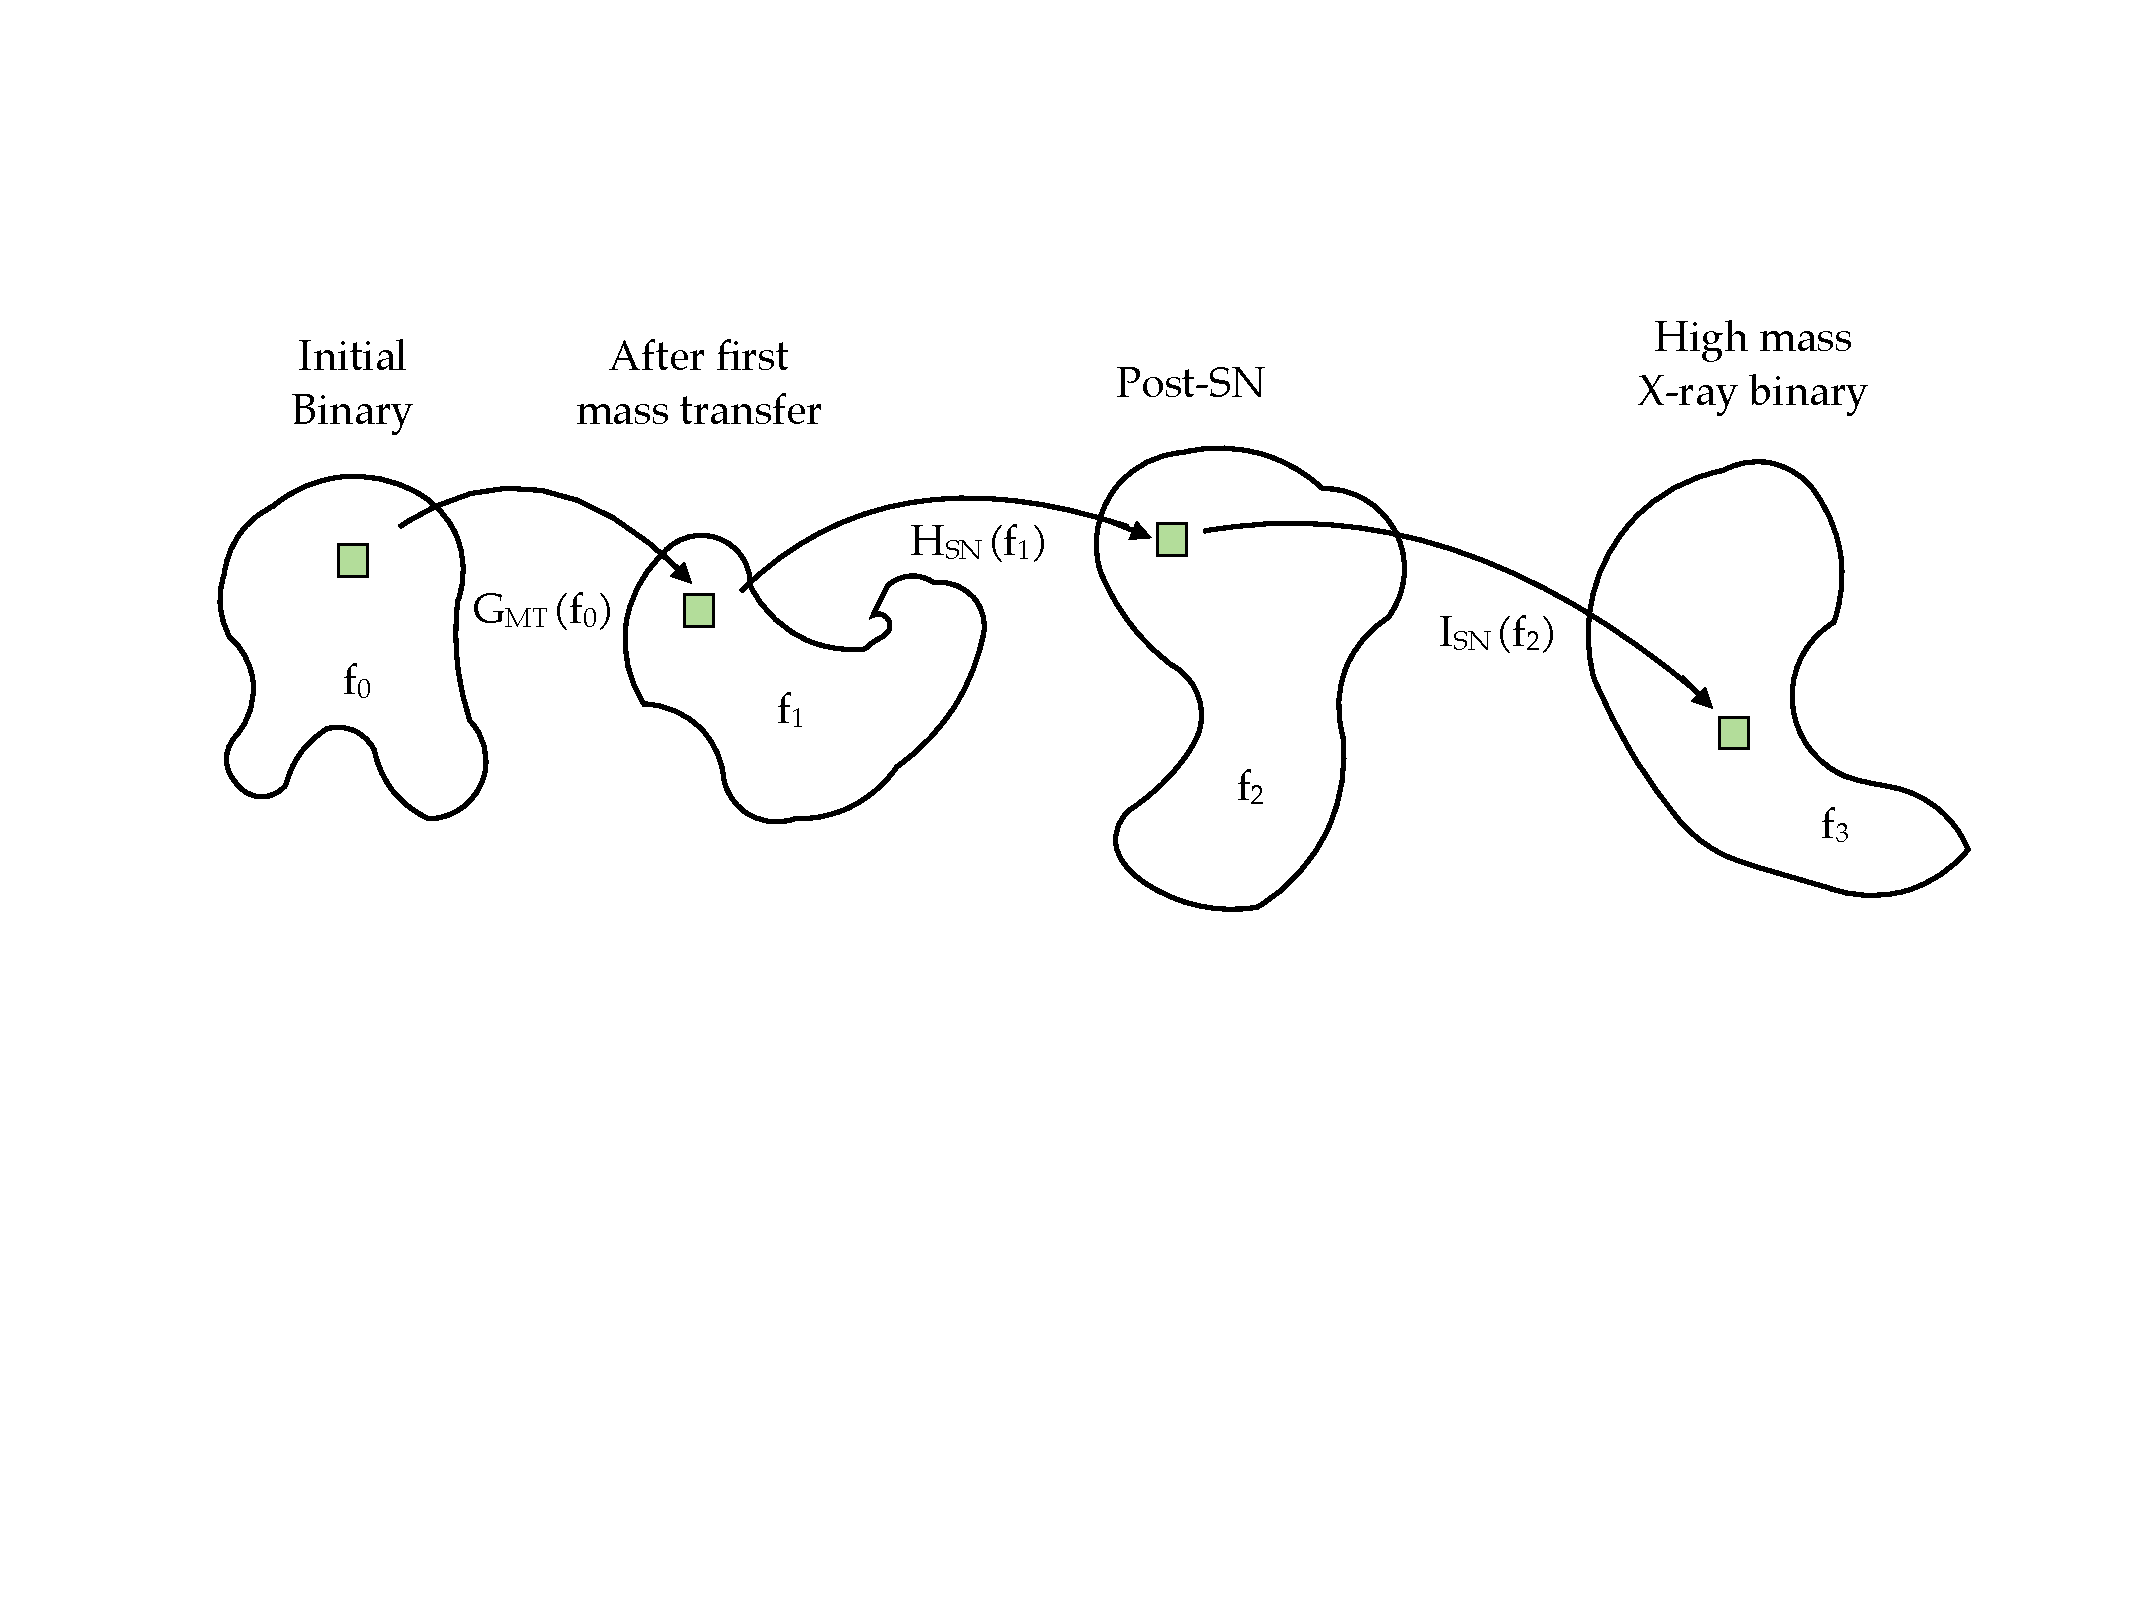
\includegraphics[width=0.95\columnwidth]{Mapping.pdf}
\caption{A mathematical representation of the evolution of a binary from its initial state three separate stages of evolution: the first (stable) mass transfer phase ($G_{\rm MT}$), the primary undergoing core collapse and receiving a natal kick ($H_{\rm SN}$), and the X-ray luminous phase once the second star evolves off the main sequence ($I_{\rm XRB}$). The volume of the three dimensional box around the binary scales with the determinant of the Jacobian matrix for each mapping.}
\label{fig:Mapping}
\end{center}
\end{figure}

Mathematically, these are mappings that can be expressed in a straightforward way:
\begin{eqnarray}
f_1 &=& G_{\rm MT} (f_0) \\
f_2 &=& H_{\rm SN} (f_1) \\
f_3 &=& I_{\rm XRB} (f_2), \\
\end{eqnarray}
which can be combined:
\begin{equation}
f_3 = I_{\rm XRB} \circ H_{\rm SN} \circ G_{\rm MT} ( f_0).
\end{equation}


If we are interesting on an individual system or a small set of binaries, we can opt for a different approach, however.


If, however, a reverse mapping exists (or it can be determined numerically), a different approach can be used. This mapping allows one to determine the initial binary state from the observed system:
\begin{equation}
f_0 = G_{\rm MT}^{-1} \circ H_{\rm SN}^{-1} \circ I_{\rm XRB}^{-1} (f_3) .
\end{equation}
Our model provides the probability of the initial state of the binary, $P(f_0)$. The series of transformations from $f_0$ to $f_3$ each shift the volume of phase space around it, affecting the resulting probability. The probability after each transition is determined by scaling the previous probability by the Jacobian of each transition. Determining the probability of the observed binary is now straightforward:
\begin{eqnarray}
P(f_3) &=& P(f_2)  J_{\rm XRB}  \\
  &=& P(f_1)  J_{\rm SN}  J_{\rm XRB}  \\
  &=& P(f_0)  J_{\rm MT}  J_{\rm SN}  J_{\rm XRB} .
\end{eqnarray}


We choose to adapt and improve upon the Jacobian formalism discussed by Kalogera (1996), Bhadkeamkar \& Ghosh (2012) and others(?). The underlying premise relies upon our ability to map the initial state of a binary through its various stages, until it forms an X-ray luminous object. If this can be done analytically or semi-analytically, such that the first partial derivatives of these mappings can be calculated, then the Jacobians of these mappings can be used to determine how the distribution of binaries evolves without having to randomly generate a population.

If we are interested in determining the probability of any particular binary with some set of observed parameters, such as the set of X-ray binaries in NGC 55, we require both the Jacobians of the three transitions defined above and the reverse mapping. Yet even the most ideal observations of high mass X-ray binaries are unlikely to identify enough parameters to uniquely determine any particular system's prior evolution. To determine the probability of any model producing a binary with observed parameters ($\vec{x}$) we marginalize over latent unobserved parameters ($\vec{y}$):
\begin{equation}
P[f_{\rm obs}(\vec{x})] = \int P[f_3(\vec{x}, \vec{y})] \dd \vec{y}.
\end{equation}
$\vec{y}$ must have enough dimensionality so that the combined $\vec{x}$ and $\vec{y}$ form a complete basis for the binary. This is the basis for the marginalization over $v_k$ and $\theta$ above in Equation \ref{eq:P_marginalized}; $L_x$, $M_2$, and $v_{\rm sys}$ alone do not form a complete basis. In principle, at least, from these five quantities, the initial masses and separation of the binary can be determined.


Below, we discuss each of the three transformations, their reverse mappings, and their Jacobian determinants.


%The reasons for this are many: including complex physics is much easier using Monte Carlo methods, the Jacobian transformation method requires the transformations to be analytic or semi-analytic whereas certain physical processes require numerical integration to accurately calculate, and Monte Carlo methods can easily handle complicated evolutionary channels. 




%Since we are only interested in a small subset of binaries, those that are strong X-ray sources, we can employ the Jacobian transformation method here. The nature of the method is significantly computational cheaper since the region of parameter space explored is, by design, limited to only those binaries we are interested in.
\end{comment}



\end{document}
